\documentclass[a4paper,12pt]{article}

\usepackage{geometry}
\geometry{a4paper, left=2.2cm, right=2.2cm, top=2.2cm, bottom=2.2cm}
\usepackage{tabularx}
\usepackage{hyperref}

\usepackage{fontspec}
\setmainfont{Times New Roman}
\usepackage{xeCJK}
\usepackage{polyglossia}
\setmainlanguage{russian} 
\setotherlanguage{chinese} 

\usepackage{graphicx}
\usepackage{amsmath}
\usepackage{listings}
\usepackage{algorithm2e} 
\usepackage{indentfirst}
\usepackage{booktabs}
\usepackage{makecell}
\usepackage{subcaption}
\usepackage{etoolbox}
\usepackage[breakable]{tcolorbox}
\usepackage{longtable}
\usepackage[export]{adjustbox}

  
\hypersetup{
    linkbordercolor=black
}

\begin{document}

\begin{titlepage}
\thispagestyle{empty}
\centering
\vspace*{1cm}
{\LARGE Московский Государственный Университет \\ имени М. В. Ломоносова \\ Механико-математический факультет \\ Кафедра МаТИС \\[2cm]}
\textbf{\huge Название статьи на русском языке}\\[0.5cm]
{\large Title of this article in English}\\[1.5cm]

{\large
\begin{tabular}{cc}
  \textit{\textbf{Author 1}} & \textit{\textbf{Author 2}}\\
  Студент 1 & Профессор 1\\
  \href{mailto:sirenexcelsior@gmail.com}{sirenexcelsior@gmail.com} & \href{mailto:exp@math.msu.ru}{exp@math.msu.ru}\\
\end{tabular}}

\vfill

\begin{figure}[htbp]
   \centering
   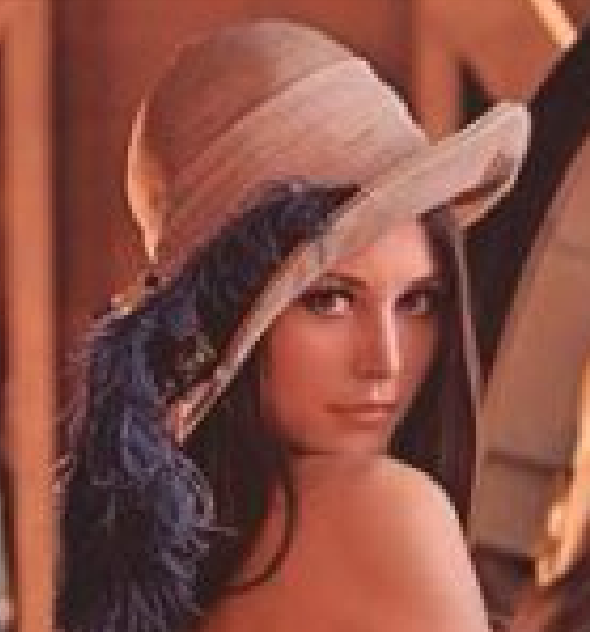
\includegraphics[width=0.6\textwidth]{pic/pic}
\end{figure}

\vfill

\large Апрель 2024 г.

\end{titlepage}

\large

\newpage
\thispagestyle{empty}
\tableofcontents

\newpage
\setcounter{page}{1}
\section{Section}

Это пример текста для заголовка, который не может быть оценен.

\subsection{Subsection}

\textbf{Это пример абзаца, выделенного жирным шрифтом.}

\textit{Это пример текста, выделенного курсивом.}

\uline{Это пример абзаца, в котором подчеркивания соединяются между строками. Если используется метод underline, текст в поперечном начертании не поддерживается.}

\subsubsection{Subsubsection}

Это пример колоночного текста.

\begin{Parallel}{0.55\textwidth}{0.4\textwidth}

\ParallelLText{

Это пример текста слева. Это образец текста слева. Это образец текста слева. Это образец текста слева. Это образец текста слева. Это образец текста слева. Это образец текста слева. Это образец текста слева.

}

\ParallelRText{

Это пример текста справа. Это образец текста справа. Это образец текста справа. Это образец текста справа. Это образец текста справа. Это образец текста справа.

}

\ParallelPar

\end{Parallel}

Это пример цитирования литературы\cite{knuth1984texbook}.

\subsubsection{Math}

Это пример математической формулы.

Это внутристрочная формула $E=mc^2$, а не межстрочная формула:

$$a^2 + b^2 = c^2$$

Вот математическая формула для автоматической нумерации, Формула \ref{eq:ft}, Формула \ref{eq:lt}, Формула \ref{eq:zt}:

\begin{equation}
F(\omega) = \int_{-\infty}^{\infty} f(t) e^{-i\omega t} \, dt
\label{eq:ft}
\end{equation}

\begin{equation}
F(s) = \int_{0}^{\infty} f(t) e^{-st} \, dt
\label{eq:lt}
\end{equation}

\begin{equation}
F(z) = \sum_{n=-\infty}^{\infty} f[n] z^{-n}
\label{eq:zt}
\end{equation}





\newpage
\section{Таблицы и рисунки}

\subsection{Таблицы}

\begin{table}[htbp]
\centering
\caption{Таблица примера}
\label{tab:t1}
\begin{tabular}{ccccc}
\toprule
Пункт & Данные 1 & Данные 2 & Данные 3 & Данные 4 \\
\midrule
	Элемент 1 & 1 & 2 \\
	Элемент 2 & 3 & 4 \\
	Элемент 3 & 5 & 6 \\
\bottomrule
\end{tabular}
\end{table}

Вот пример вставки и ссылки на трехстрочную таблицу \ref{tab:t1}.

\subsection{Рисунки}

\begin{figure}[htbp]
    \centering
    \begin{subfigure}[b]{0.3\textwidth}
        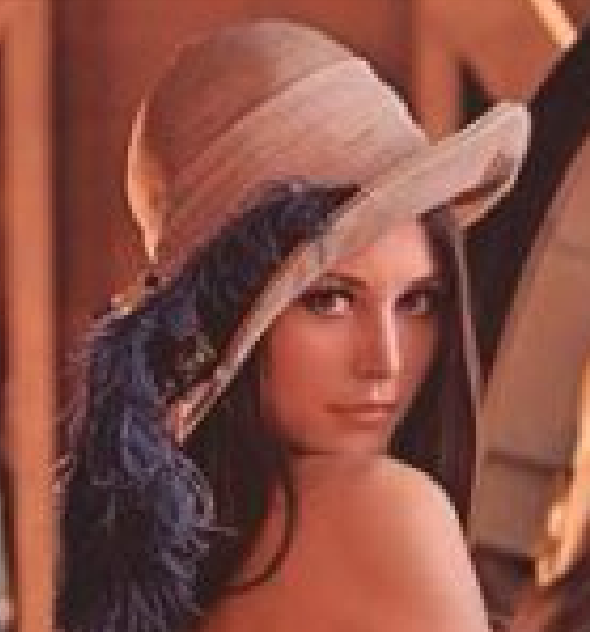
\includegraphics[width=\textwidth]{pic/pic} 
        \caption{Рис 1-1}
        \label{fig:sub1}
    \end{subfigure}
    \hfill 
    \begin{subfigure}[b]{0.3\textwidth}
        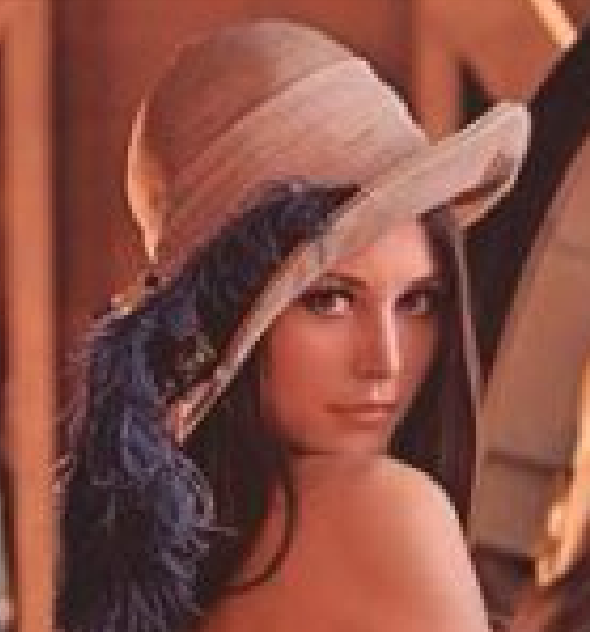
\includegraphics[width=\textwidth]{pic/pic} 
        \caption{Рис 1-2}
        \label{fig:sub2}
    \end{subfigure}
    \hfill 
    \begin{subfigure}[b]{0.3\textwidth}
        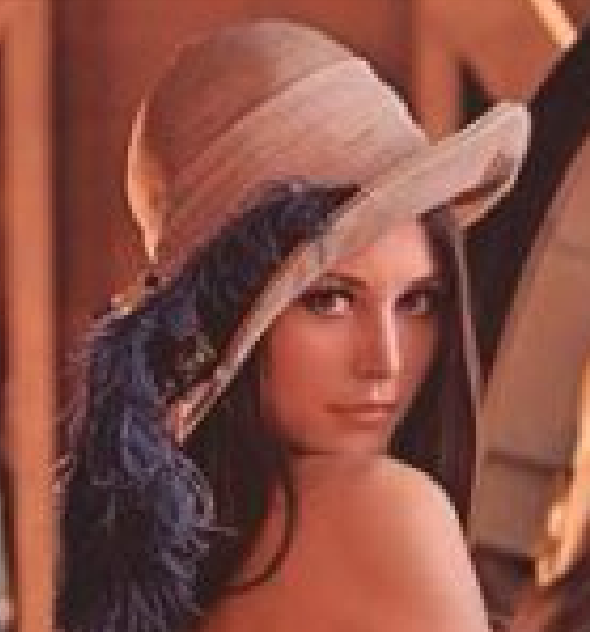
\includegraphics[width=\textwidth]{pic/pic} 
        \caption{Рис 1-3}
        \label{fig:sub3}
    \end{subfigure}
    \caption{Примеры картинок}
    \label{fig:total}
\end{figure}

Вот пример вставки и ссылки на изображение \ref{fig:total} и \ref{fig:sub1}, \ref{fig:sub2}, \ref{fig:sub3}.



\newpage
\section{Код}

\begin{lstlisting}[language=Python]
import numpy as np

def inc(x):
    # Increase a number by 1.
    return x + 1

arr = np.array([1, 2, 3])
print(inc(arr))
\end{lstlisting}

Это пример представления кода.



\bibliographystyle{plain}
\bibliography{references}
\addcontentsline{toc}{section}{Список литературы}

\end{document}

